% Changed from the snippet that this document comes from: added the \documentclass line, and removed
% two blank lines inside the axis options (a blank line there is a \par, which
% pdfLaTeX rejects with "Paragraph ended before ... was complete").
\documentclass{standalone}
\usepackage{tikz}
\usetikzlibrary{shapes,arrows,positioning,calc,fit,arrows.meta,decorations.markings}
\usepackage{pgfplots}
\pgfplotsset{compat=1.16}

\newcommand*{\TickSize}{4pt}
\newcommand*{\bfreq}{2}
\newcommand*{\B}{3}

\begin{document}
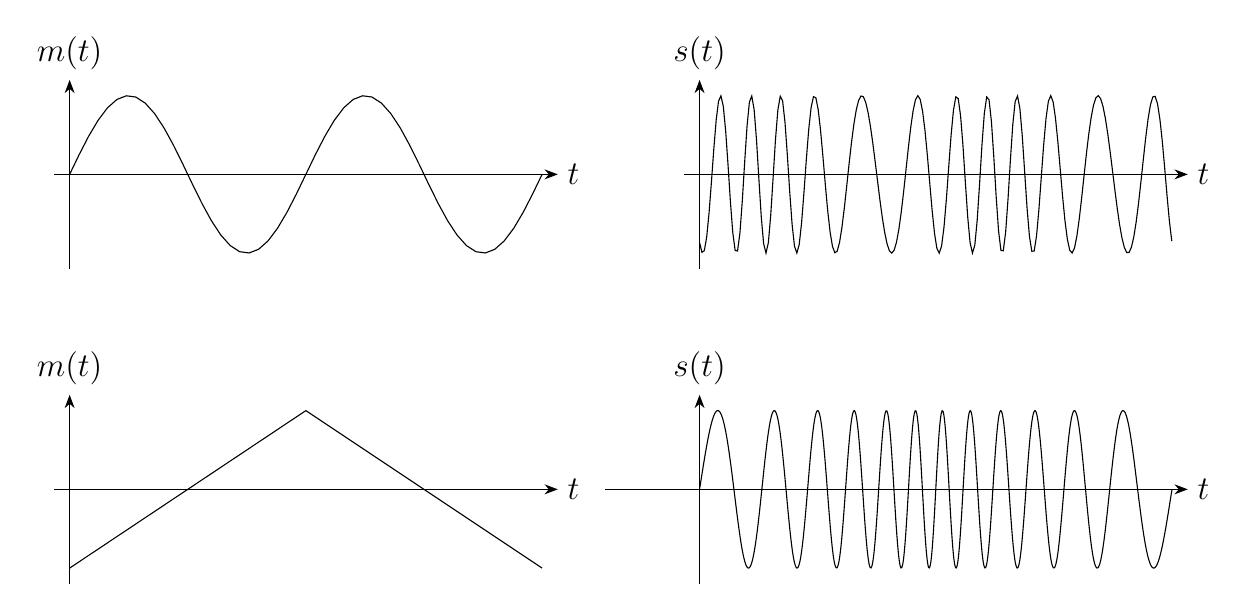
\begin{tikzpicture}[font=\large, domain=0:6, samples=51,>={Stealth}]
	\begin{scope}[shift={(0,0)}]
		\draw[->] (-0.2,0) -- (6.2,0) node[right] {$t$};
		\draw[->] (0,-1.2) -- (0,1.2) node[above] {$m(t)$};

		\draw[] plot (\x,{sin(\x*120)});
	\end{scope}
	\begin{scope}[shift={(8,0)}]
		\draw[->] (-0.2,0) -- (6.2,0) node[right] {$t$};
		\draw[->] (0,-1.2) -- (0,1.2) node[above] {$s(t)$};

		\draw[samples=200] plot (\x,{sin((\x - (0.5/\B)*cos(\x*120))*\bfreq*360)});
	\end{scope}

	\begin{scope}[shift={(0,-4)}]
		\draw[->] (-0.2,0) -- (6.2,0) node[right] {$t$};
		\draw[->] (0,-1.2) -- (0,1.2) node[above] {$m(t)$};

		\draw[] plot (\x, {1 - (abs(\x-\B)*2/\B)});
	\end{scope}
	\begin{scope}[shift={(8,-4)}]
		\draw[->] (-1.2,0) -- (6.2,0) node[right] {$t$};
		\draw[->] (0,-1.2) -- (0,1.2) node[above] {$s(t)$};

	    \begin{axis}[
			at={(0,0)},
			anchor=west,
			height=2cm,
			width=6cm,
			scale only axis,
		    enlargelimits=false,
		    clip=false,
			axis lines=none,
		    ticks=none,
			samples=300,
			smooth,
	    ]
		    - \addplot[domain=0:\B] {sin((x + 0.5*(((x^2)/\B)-x))*\bfreq*360)};
		    \addplot[domain=\B:2*\B] {sin((x + 0.5*(3*x-((x^2)/\B)-2*\B))*\bfreq*360)};
		\end{axis}
	\end{scope}
\end{tikzpicture}
\end{document}
